% !TEX program = xelatex
\documentclass[10pt,aspectratio=169]{beamer}
\usepackage{fontspec}
\usepackage{amsmath,amssymb,mathtools}
\usepackage{tikz}
\usetikzlibrary{arrows.meta,positioning}
\IfFontExistsTF{DejaVu Sans}{
  \setmainfont{DejaVu Sans}
  \setsansfont{DejaVu Sans}
}{
  \setmainfont{Arial}
  \setsansfont{Arial}
}
\usefonttheme{professionalfonts}
\definecolor{ink}{HTML}{1F2A40}
\definecolor{blue}{HTML}{225FA5}
\definecolor{teal}{HTML}{0E827A}
\definecolor{graytext}{HTML}{677489}
\definecolor{paleblue}{HTML}{EDF4FB}
\definecolor{paleteal}{HTML}{ECF7F4}
\definecolor{lightline}{HTML}{DCE4EA}
\setbeamercolor{normal text}{fg=ink,bg=white}
\setbeamercolor{structure}{fg=teal}
\setbeamercolor{frametitle}{fg=ink,bg=white}
\setbeamercolor{block title}{fg=blue,bg=paleblue}
\setbeamercolor{block body}{fg=ink,bg=paleblue}
\setbeamerfont{frametitle}{size=\large,series=\bfseries}
\setbeamertemplate{navigation symbols}{}
\setbeamertemplate{itemize item}{\color{teal}$\blacktriangleright$}
\setbeamertemplate{frametitle}{\vspace{0.28cm}\insertframetitle\par\vspace{0.07cm}{\color{teal}\rule{\textwidth}{0.65pt}}}
\setbeamertemplate{footline}{\hspace{0.55cm}{\tiny\color{graytext}\insertshorttitle}\hfill{\tiny\color{graytext}\insertframenumber/\inserttotalframenumber}\hspace{0.55cm}\vspace{0.22cm}}
\setbeamersize{text margin left=0.73cm,text margin right=0.73cm}
\newcommand{\src}[1]{\vfill{\tiny\color{graytext}Gu et al., arXiv:2109.03992, #1}}
\newcommand{\nsfsrc}[1]{\vfill{\tiny\color{graytext}Kiyohara, Johns, Li, NeurIPS 2025, arXiv:2510.25769, #1}}
\newcommand{\dynsrc}[1]{\vfill{\tiny\color{graytext}A. Zhu, Q. Li, DynGMA, arXiv:2402.14475 (2024), #1}}
\tikzset{flow/.style={draw=lightline,very thick,rounded corners=3pt,fill=paleblue,align=center,inner sep=7pt,minimum height=1.22cm,font=\small}, done/.style={flow,fill=paleteal}, arrow/.style={-{Stealth[length=2.8mm]},line width=1pt,draw=teal}}
\title[Нейросетевые методы для стохастического ряда]{Нейросетевые методы для одномерного стохастического ряда}
\begin{document}

\begin{frame}[plain]
\vspace{1cm}{\color{teal}\rule{1.9cm}{2.5pt}}\par\vspace{0.6cm}
{\huge\bfseries Нейросетевые методы\\[0.2cm] для СДУ Ито}\par\vspace{0.5cm}
{\large Общая постановка задачи и три подхода из литературы}\par\vspace{0.5cm}
{\color{graytext}Одномерный случай; без физической интерпретации}\par\vfill
{\footnotesize\color{graytext}Статья 1: Y. Gu, J. Harlim, S. Liang, H. Yang,\\
\textit{Stationary Density Estimation of It\^o Diffusions Using Deep Learning}, 2021.\\
\textcolor{blue}{\url{https://arxiv.org/abs/2109.03992}}}\\[0.08cm]
{\footnotesize\color{graytext}Статья 2: N. Kiyohara, E. Johns, Y. Li. \textit{Neural Stochastic Flows}, NeurIPS 2025.\\
\textcolor{blue}{\url{https://arxiv.org/abs/2510.25769}}}\\[0.08cm]
{\footnotesize\color{graytext}Статья 3: A. Zhu, Q. Li. \textit{DynGMA: a robust approach for learning SDEs from data}, 2024.\\
\textcolor{blue}{\url{https://arxiv.org/abs/2402.14475}}}\vspace{0.18cm}
\end{frame}

\begin{frame}{Общая задача}
\vspace{0.15cm}
\begin{block}{Цель}
Построить \textbf{нейросетевой вероятностный прогноз} по наблюдениям и проверить его \textbf{надёжность на длинных горизонтах}.
\end{block}
\vspace{0.17cm}
\begin{enumerate}\setlength\itemsep{0.21cm}
\item Подготовить временной ряд и данные для обучения/проверки.
\item Обучить модель динамики; в общей постановке предусмотреть коррекцию по наблюдениям.
\item Получать ансамбль прогнозов и оценивать неопределённость.
\item Исследовать устойчивость и предельные распределения.
\item Сравнить с классической моделью по точности и затратам.
\end{enumerate}
\vfill{\tiny\color{graytext}Основа: «Задача.txt», пункты 1--5; здесь -- сознательное упрощение до одномерного ряда.}
\end{frame}

\begin{frame}{Математическая постановка первого этапа}
\vspace{0.13cm}
\begin{center}
{\Large $dX_t=a(X_t)\,dt+b(X_t)\,dW_t$}
\end{center}
\vspace{0.16cm}
Дано: дискретные наблюдения $x_0,x_1,\dots,x_N$ с шагом $\Delta t$; $a,b$ неизвестны.
\vspace{0.2cm}
\begin{columns}[T,onlytextwidth]
\begin{column}{0.47\textwidth}
\textcolor{blue}{\bfseries Вероятностный прогноз}\par\vspace{0.17cm}
$\displaystyle p_\Delta(y\mid x)=p(X_{t+\Delta t}=y\mid X_t=x)$\par\vspace{0.17cm}
Нужен для прогноза и ансамблей.
\end{column}
\begin{column}{0.47\textwidth}
\textcolor{teal}{\bfseries Долгосрочная статистика}\par\vspace{0.17cm}
$\displaystyle p_\infty(x)=\lim_{t\to\infty}p(t,x)$\par\vspace{0.17cm}
Нужна для анализа устойчивости.
\end{column}
\end{columns}
\vspace{0.28cm}
\begin{block}{Что решает статья Gu et al.}
Именно \textbf{вторую задачу}: восстановление стационарной плотности $p_\infty$ по временному ряду при предположении эргодичности.
\end{block}
\end{frame}


\begin{frame}{Обозначения: общая постановка}
\vspace{0.02cm}
{\small
\begin{columns}[T,onlytextwidth]
\begin{column}{0.49\textwidth}
\begin{tabular}{@{}p{1.45cm}p{4.7cm}@{}}
$X_t$ & случайный процесс \\[0.08cm]
$x_i$ & значение ряда в момент $t_i$ \\[0.08cm]
$W_t$ & винеровский процесс \\[0.08cm]
$a(x)$ & коэффициент сноса \\[0.08cm]
$b(x)$ & амплитуда шума \\[0.08cm]
$\Delta$ & временной интервал $t-s$
\end{tabular}
\end{column}
\begin{column}{0.49\textwidth}
\begin{tabular}{@{}p{2.0cm}p{4.1cm}@{}}
$q_\Delta(y\mid x)$ & переходная плотность \\[0.08cm]
$p(t,y)$ & плотность $X_t$ \\[0.08cm]
$p_\infty(y)$ & предельная плотность \\[0.08cm]
$\theta,\phi,\eta,\xi$ & веса разных сетей \\[0.08cm]
$\mathcal L$ & функция потерь \\[0.08cm]
$L$ & слои / шаги (контекст)
\end{tabular}
\end{column}
\end{columns}}
\vspace{0.10cm}
\begin{block}{Разница двух плотностей}
$q_\Delta(y\mid x)$ задаёт \textbf{переход из состояния $x$};
$p_\infty(y)$ описывает \textbf{долгосрочную статистику} и существует не всегда.
\end{block}
\end{frame}

\begin{frame}{Gu et al.: базовая концепция}
\vspace{0.25cm}
\begin{center}
\begin{tikzpicture}[node distance=0.34cm]
\node[flow,text width=2.1cm] (series) {Наблюдения\\$x_0,\ldots,x_N$};
\node[flow,right=of series,text width=2.55cm] (coeff) {\textbf{Шаг 1}\\Нейросети\\$a_\theta(x),\ B_\phi(x)$};
\node[flow,right=of coeff,text width=2.65cm] (fp) {\textbf{Шаг 2}\\Стационарное\\Фоккера--Планка};
\node[done,right=of fp,text width=1.6cm] (p) {$p_\eta(x)$\\плотность};
\draw[arrow] (series)--(coeff);\draw[arrow] (coeff)--(fp);\draw[arrow] (fp)--(p);
\end{tikzpicture}
\end{center}
\vspace{0.2cm}
\begin{itemize}\setlength\itemsep{0.23cm}
\item \textbf{Сначала} идентифицируется стохастическая динамика: $a(x)$ и $B(x)=b^2(x)$.
\item \textbf{Затем} третья нейросеть аппроксимирует стационарную плотность как решение PDE.
\end{itemize}
\src{\S\S 2--3, формулы (1)--(3), (6)--(13)}
\end{frame}


\begin{frame}{Gu et al.: обозначения параметров}
\vspace{0.10cm}
\begin{columns}[T,onlytextwidth]
\begin{column}{0.49\textwidth}
\textcolor{blue}{\bfseries Модель коэффициентов}
\begin{align*}
 a_\theta(x)&\approx a(x),\\
 B_\phi(x)&\approx b^2(x).
\end{align*}
$\theta$ --- веса сети сноса.\\[0.13cm]
$\phi$ --- веса сети квадрата диффузии.
\end{column}
\begin{column}{0.49\textwidth}
\textcolor{teal}{\bfseries Модель плотности}
\begin{align*}
 p_\eta(x)&\approx p_\infty(x),\\
 \mathcal L_p(\eta)&\longrightarrow\min.
\end{align*}
$\eta$ --- веса сети плотности.\\[0.13cm]
$\lambda_1,\lambda_2$ --- веса ограничений в $\mathcal L_p$.
\end{column}
\end{columns}
\vspace{0.25cm}
\begin{block}{Не путать}
$B(x)=b^2(x)$ --- \textbf{дисперсия шума в единицу времени};
$\theta,\phi,\eta$ --- не значения $X_t$, а настраиваемые веса разных нейросетей.
\end{block}
\src{\S 3.2--3.3, формулы (6), (9), (10)--(17)}
\end{frame}

\begin{frame}{Шаг 1а: восстановление сноса}
\vspace{0.11cm}
\begin{align*}
\Delta X_n&=X_{n+1}-X_n\approx a(X_n)\Delta t+b(X_n)\sqrt{\Delta t}\,\xi_n,\\
Y_n&=\frac{X_{n+1}-X_n}{\Delta t},\quad \xi_n\sim\mathcal N(0,1).
\end{align*}
\vspace{0.03cm}
\begin{center}
\large $\displaystyle\boxed{\mathcal L_a(\theta)=\frac1N\sum_{n=0}^{N-1}\bigl(Y_n-a_\theta(X_n)\bigr)^2}$
\end{center}
\vspace{0.17cm}
\begin{block}{Идея}
$\mathbb E[Y_n\mid X_n=x]\approx a(x)$. Обучение сводится к обычной регрессии по приращениям ряда.
\end{block}
\src{\S 3.2, формулы (3), (5)--(7)}
\end{frame}

\begin{frame}{Шаг 1б: восстановление диффузии}
\vspace{0.12cm}
После оценки $a_\theta$ берём остатки $r_n=Y_n-a_\theta(X_n)$.
\begin{center}
\large $\displaystyle\boxed{\mathcal L_B(\phi)=\frac1N\sum_{n=0}^{N-1}\left(\Delta t\,r_n^2-B_\phi(X_n)\right)^2}$
\end{center}
\vspace{0.2cm}
\begin{columns}[T,onlytextwidth]
\begin{column}{0.49\textwidth}
\textcolor{blue}{\bfseries Вариант A: $B(x)$ неизвестная функция}\par\vspace{0.16cm}
Обучаем отдельную сеть $B_\phi(x)\approx b^2(x)$.
\end{column}
\begin{column}{0.48\textwidth}
\textcolor{teal}{\bfseries Вариант B: $B(x)=\sigma^2$ постоянна}\par\vspace{0.16cm}
$\displaystyle\widehat{\sigma^2}=\frac{\Delta t}{N}\sum_{n=0}^{N-1}r_n^2$.\par\vspace{0.1cm}
Вторая сеть не нужна.
\end{column}
\end{columns}
\src{\S 3.2, формулы (8)--(9); функция потерь масштабирована на $\Delta t^2$}
\end{frame}

\begin{frame}[shrink=4]{Шаг 2: стационарная плотность}
\vspace{0.06cm}
Заменяем неизвестные коэффициенты на $a_\theta$ и $B_\phi$:
\begin{center}
$\displaystyle \boxed{\widehat{\mathcal L}^{\!*}p_\eta(x)=-\frac{d}{dx}(a_\theta p_\eta)+\frac12\frac{d^2}{dx^2}(B_\phi p_\eta)\approx0}$
\end{center}
\vspace{0.1cm}
На ограниченной области $\Omega=[-R,R]$ обучаем третью сеть:
\vspace{-0.1cm}
\begin{align*}
\mathcal L_p(\eta)={}&\int_\Omega |\widehat{\mathcal L}^{\!*}p_\eta|^2dx
+\lambda_1\left(\int_\Omega p_\eta\,dx-1\right)^2\\
&+\lambda_2\Vert p_\eta\Vert_{L^2(\partial\Omega)}^2.
\end{align*}
\vspace{-0.10cm}
\begin{block}{Численная реализация из статьи}
Интегралы: квадратуры или Монте-Карло. Дополнительно контролируют нормировку, границу и положительность.
\end{block}
\src{\S 3.3, формулы (10)--(17)}
\end{frame}

\begin{frame}{Какие варианты действительно рассматривает статья}
\vspace{0.08cm}
\begin{enumerate}\setlength\itemsep{0.28cm}
\item \textbf{Оценка диффузии:} сеть $B_\phi(x)$ или постоянная матрица/константа по остаткам (\S 3.2).
\item \textbf{Архитектура:} полносвязная сеть (FNN) или ResNet для аппроксимации коэффициентов (\S 3.1, 5).
\item \textbf{Обучение плотности:} невзвешенный остаток PDE на $\Omega$ или взвешенный по эмпирическим точкам ряда (\S 3.3, 5).
\item \textbf{Интегрирование:} Монте-Карло; в малой размерности возможны квадратуры (\S 3.3).
\end{enumerate}
\vspace{0.18cm}
\begin{block}{Не рассматривается в этой статье}
Прямое обучение $p(X_{t+\Delta t}\mid X_t)$ и эволюции $p(t,x)$: это другие задачи.
\end{block}
\end{frame}

\begin{frame}{Что можем сделать в 1D на первом этапе}
\vspace{0.17cm}
\begin{center}
\begin{tikzpicture}[node distance=0.31cm]
\node[flow,text width=2.0cm] (gen) {Ряд из простого\\СДУ Ито};
\node[flow,right=of gen,text width=2.2cm] (fit) {Обучить\\$a_\theta,\ B_\phi$};
\node[flow,right=of fit,text width=2.5cm] (neural) {Найти $p_\eta$\\из стационарного PDE};
\node[done,right=of neural,text width=1.9cm] (test) {Сравнить\\с эталоном};
\draw[arrow] (gen)--(fit);\draw[arrow] (fit)--(neural);\draw[arrow] (neural)--(test);
\end{tikzpicture}
\end{center}
\vspace{0.2cm}
\textbf{Простой тест:} $dX_t=-\kappa X_tdt+\sigma dW_t$, $\kappa>0$.
\begin{center}
$\displaystyle p_\infty(x)=\sqrt{\frac{\kappa}{\pi\sigma^2}}\exp\!\left(-\frac{\kappa x^2}{\sigma^2}\right)$
\end{center}
\vspace{0.08cm}
\textbf{Проверить:} коэффициенты $a,B$; нормировку $p_\eta$; ошибку плотности и статистику длинных траекторий.
\vspace{0.1cm}
{\small\color{teal}\bfseries Это предлагаемый нами эксперимент, не пример из статьи.}
\src{Примеры авторов: \S 5, двумерное распределение Стьюдента и 20D Langevin}
\end{frame}

\begin{frame}{Подход Gu et al.: итог и ограничения}
\vspace{0.22cm}
\begin{block}{Практический результат}
Метод позволяет по одному дискретному ряду оценить $a(x)$, $b^2(x)$ и \textbf{стационарную плотность} $p_\infty(x)$.
\end{block}
\vspace{0.15cm}
\begin{itemize}\setlength\itemsep{0.28cm}
\item Требуются эргодичность и корректность стохастической модели.
\item Влияют ошибки дискретизации, регрессии коэффициентов и решения PDE.
\item Для условной плотности $p(X_{t+\Delta t}\mid X_t)$ рассмотрим другой метод: Neural Stochastic Flows.
\end{itemize}
\vfill
{\small\bfseries Источник:} {\small Y. Gu, J. Harlim, S. Liang, H. Yang.\ \textit{Stationary Density Estimation of It\^o Diffusions Using Deep Learning}. 2021.\ \url{https://arxiv.org/abs/2109.03992}}
\end{frame}


% ---------- SECOND PAPER: NEURAL STOCHASTIC FLOWS ----------
\begin{frame}{Подход 2: Neural Stochastic Flows (NSF)}
\vspace{0.04cm}
\begin{block}{Идея статьи Kiyohara, Johns, Li (2025)}
Обучать \textbf{не коэффициенты СДУ}, а непосредственно \textbf{переходную плотность} $p_\theta(x_t\mid x_s;\,t-s)$ без численного решения СДУ.
\end{block}
\vspace{0.10cm}
\begin{center}
\begin{tikzpicture}[node distance=0.32cm]
\node[flow,text width=2.0cm] (inp) {Состояние $x_s$\\интервал $\Delta=t-s$};
\node[flow,right=of inp,text width=2.45cm] (g) {Шум $\varepsilon\sim\mathcal N(0,1)$\\условный flow};
\node[done,right=of g,text width=2.25cm] (out) {$x_t=F_\theta(x_s,\Delta,\varepsilon)$};
\node[done,right=of out,text width=1.76cm] (dens) {$p_\theta(x_t\mid x_s;\Delta)$};
\draw[arrow] (inp)--(g);\draw[arrow] (g)--(out);\draw[arrow] (out)--(dens);
\end{tikzpicture}
\end{center}
\vspace{0.14cm}
\begin{itemize}\setlength\itemsep{0.14cm}
\item \textbf{Normalizing flow:} обратимые преобразования позволяют вычислять плотность.
\item Переход на произвольный $\Delta$ внутри обученного горизонта --- за один вызов сети.
\end{itemize}
\nsfsrc{\S\S 1, 3; рис. 1; формулы (2)--(3)}
\end{frame}


\begin{frame}{NSF: обозначения и параметры}
\vspace{0.03cm}
{\small
\begin{columns}[T,onlytextwidth]
\begin{column}{0.49\textwidth}
\begin{tabular}{@{}p{2.15cm}p{3.95cm}@{}}
$s<t$ & начало / конец \\[0.07cm]
$\Delta=t-s$ & горизонт прогноза \\[0.07cm]
$c=(x_s,\Delta)$ & условие модели \\[0.07cm]
$\varepsilon$ & стандартный нормальный шум \\[0.07cm]
$z$ & базовая случайная величина
\end{tabular}
\end{column}
\begin{column}{0.49\textwidth}
\begin{tabular}{@{}p{1.65cm}p{4.45cm}@{}}
$F_\theta$ & обратимое преобразование \\[0.07cm]
$\theta$ & веса основной сети \\[0.07cm]
$q_\theta$ & переходная плотность \\[0.07cm]
$L$ & число слоёв flow \\[0.07cm]
$\mathcal L$ & функция потерь
\end{tabular}
\end{column}
\end{columns}}
\vspace{0.13cm}
\begin{block}{Если динамика зависит от абсолютного времени}
Во входы добавляют время начала: $c=(x_s,s,\Delta)$.
\end{block}
\nsfsrc{\S 3.1, формулы (3), (5)--(7)}
\end{frame}

\begin{frame}{NSF: свойства переходной плотности}
\vspace{0.06cm}
Для $s<u<t$ обозначим $q_\theta(y\mid x;s,t)=p_\theta(X_t=y\mid X_s=x)$.
\vspace{0.17cm}
\begin{align*}
\text{Тождественность: }&\quad q_\theta(y\mid x;s,s)=\delta(y-x),\\[0.13cm]
\text{Чепмен--Колмогоров: }&\quad
q_\theta(z\mid x;s,t)=\int_{\mathbb R}q_\theta(z\mid y;u,t)
q_\theta(y\mid x;s,u)\,dy.
\end{align*}
\vspace{0.02cm}
\begin{block}{Автономное СДУ}
При $a=a(x)$ и $b=b(x)$ переходное ядро \textbf{не зависит от начального времени}: $q_\theta(y\mid x;s,t)=q_\theta(y\mid x;\,t-s)$.
\end{block}
\vspace{0.08cm}
\small \textcolor{teal}{\bfseries Важно:} временная однородность переходов не означает существования стационарной плотности $p_\infty$.
\nsfsrc{\S 3, формула (4), свойства identity / Markov / stationarity}
\end{frame}

\begin{frame}{Как устроена модель NSF}
\vspace{0.06cm}
\textbf{Базовое распределение} (здесь показана одномерная запись):
\begin{center}
$\displaystyle z=x_s+\Delta\,m_\theta(x_s,\Delta)
+\sqrt{\Delta}\,s_\theta(x_s,\Delta)\varepsilon,
\quad\varepsilon\sim\mathcal N(0,1).$
\end{center}
\vspace{0.08cm}
\textbf{Преобразование:} $\displaystyle x_t=F_\theta(z;\,x_s,\Delta)$, где $F_\theta$ обратимо.
\vspace{0.12cm}
\begin{block}{Оригинальная многомерная архитектура}
Авторы применяют \textbf{affine coupling layers}: для разбиения $z=(z_A,z_B)$
\[
 z'_A=z_A,\qquad
 z'_B=z_B\odot\exp\{\Delta S_\theta(z_A,c)\}+\Delta T_\theta(z_A,c).
\]
При $\Delta=0$: базовое распределение вырождается в $x_s$, преобразование становится тождественным.
\end{block}
\vspace{0.01cm}
\small\textcolor{teal}{\bfseries Особенность 1D:} обычное разбиение $z_A,z_B$ для скалярного состояния неприменимо; нужен отдельный одномерный обратимый flow (наша адаптация).
\nsfsrc{\S 3.1, формулы (5)--(7); приложение A.1}
\end{frame}

\begin{frame}{Почему плотность вычисляется явно}
\vspace{0.11cm}
Пусть $z\sim\mathcal N(\mu_\theta,\sigma_\theta^2)$ и
$y=F_\theta(z;c)$, $c=(x_s,\Delta)$.
\vspace{0.14cm}
Для обратимого дифференцируемого $F_\theta$:
\[
\boxed{\quad p_\theta(y\mid x_s;\Delta)
=\frac{\mathcal N\!\left(F_\theta^{-1}(y;c);\mu_\theta,\sigma_\theta^2\right)}
{\left|\partial_zF_\theta\!\left(F_\theta^{-1}(y;c);c\right)\right|}.\quad}
\]
\vspace{0.08cm}
\begin{block}{Обучение по наблюдаемым парам}
Для набора $\mathcal D=\{(x_{t_i},x_{t_j},\Delta_{ij})\}$:
\[
\mathcal L_{\mathrm{NLL}}(\theta)=-\frac{1}{|\mathcal D|}
\sum_{(i,j)\in\mathcal D}\log p_\theta(x_{t_j}\mid x_{t_i};\Delta_{ij}).
\]
\end{block}
\nsfsrc{\S 3.1--3.2, формула (11); приложение D, формула (36)}
\end{frame}

\begin{frame}{Согласованность прогнозов на разных горизонтах}
\vspace{0.02cm}
\begin{center}
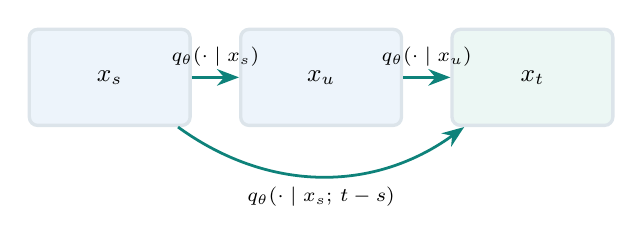
\begin{tikzpicture}[node distance=0.6cm]
\node[flow,text width=1.55cm] (x) {$x_s$};
\node[flow,right=of x,text width=1.55cm] (y) {$x_u$};
\node[done,right=of y,text width=1.55cm] (z) {$x_t$};
\draw[arrow] (x)--node[above,font=\scriptsize]{$q_\theta(\cdot\mid x_s)$}(y);
\draw[arrow] (y)--node[above,font=\scriptsize]{$q_\theta(\cdot\mid x_u)$}(z);
\draw[arrow,bend right=36] (x) to node[below,font=\scriptsize]{$q_\theta(\cdot\mid x_s;\,t-s)$}(z);
\end{tikzpicture}
\end{center}
\vspace{0.07cm}
\textbf{Задача:} согласовать прямой прогноз $s\to t$ и составной $s\to u\to t$.
\[
q_\theta^{(2)}(z\mid x)=\int q_\theta(z\mid y;u,t)
q_\theta(y\mid x;s,u)\,dy.
\]
\vspace{-0.06cm}
\begin{block}{Функция потерь из статьи}
$\displaystyle \mathcal L_{\mathrm{total}}=\mathcal L_{\mathrm{NLL}}+
\lambda\mathcal L_{\mathrm{flow}}$,
где $\mathcal L_{\mathrm{flow}}$ минимизирует \textbf{вариационные верхние оценки} двух направлений KL:
$D_{\rm KL}(q^{(1)}\Vert q^{(2)})$ и $D_{\rm KL}(q^{(2)}\Vert q^{(1)})$.
\end{block}
\nsfsrc{\S 3.2, формулы (4), (8)--(11); рис. 1(c,d)}
\end{frame}

\begin{frame}[shrink=5]{Как вычисляют $\mathcal L_{\mathrm{flow}}$}
\vspace{0.08cm}
Поскольку $q^{(2)}$ содержит интеграл по $x_u$, вводится \textbf{мостовая сеть}
$\,b_\xi(x_u\mid x_s,x_t)$ для промежуточного состояния.
\vspace{0.14cm}
\textbf{Прямое направление (1 $\to$ 2):}
\[
\mathcal L_{1\to2}=
\mathbb E_{x_t\sim q^{(1)},\,x_u\sim b_\xi}
\log\frac{q^{(1)}(x_t\mid x_s)\,b_\xi(x_u\mid x_s,x_t)}
{q_\theta(x_t\mid x_u)\,q_\theta(x_u\mid x_s)}.
\]
\textbf{Обратное направление (2 $\to$ 1):}
\[
\mathcal L_{2\to1}=
\mathbb E_{x_u\sim q_\theta(\cdot\mid x_s),\,x_t\sim q_\theta(\cdot\mid x_u)}
\log\frac{q_\theta(x_u\mid x_s)\,q_\theta(x_t\mid x_u)}
{b_\xi(x_u\mid x_s,x_t)\,q^{(1)}(x_t\mid x_s)}.
\]
\vspace{0.02cm}
\small Итого: $\displaystyle\mathcal L_{\mathrm{flow}}=\mathbb E_{s<u<t}[\mathcal L_{1\to2}+\mathcal L_{2\to1}]$.
\nsfsrc{\S 3.2, формулы (8)--(10); приложения A.2 и B}
\end{frame}


\begin{frame}{NSF: что такое мостовая сеть $b_\xi$?}
\vspace{0.13cm}
\begin{center}
\begin{tikzpicture}[node distance=0.68cm]
\node[flow,text width=1.75cm] (x) {Известно\\$X_s=x_s$};
\node[flow,right=of x,text width=2.35cm] (u) {Неизвестно\\$X_u$, $s<u<t$};
\node[done,right=of u,text width=1.75cm] (y) {Известно\\$X_t=x_t$};
\draw[arrow] (x) -- (u); \draw[arrow] (u) -- (y);
\end{tikzpicture}
\end{center}
\vspace{0.13cm}
\begin{center}
$\displaystyle \boxed{\ b_\xi(x_u\mid x_s,x_t;s,u,t)\approx
 p(X_u=x_u\mid X_s=x_s,X_t=x_t)\ }$
\end{center}
\vspace{0.15cm}
\begin{itemize}\setlength\itemsep{0.13cm}
\item $\xi$ --- \textbf{веса вспомогательной нейросети}, а не коэффициент диффузии $b(x)$ в СДУ.
\item Мостовая сеть выдаёт \textbf{распределение возможного промежуточного состояния} при фиксированных концах.
\item Нужна для вычислимой регуляризации согласованности «прямой переход = два перехода».
\end{itemize}
\nsfsrc{\S 3.2, формулы (8)--(10); приложение A.2, формулы (19)--(21)}
\end{frame}

\begin{frame}{Второй вариант из статьи: Latent NSF}
\vspace{0.12cm}
При \textbf{неполных или зашумлённых наблюдениях} $o_{t_i}$ вводится скрытое состояние $z_{t_i}$.
\vspace{0.16cm}
\begin{center}
\begin{tikzpicture}[node distance=0.36cm]
\node[flow,text width=2.1cm] (obs) {Наблюдения $o_{t_i}$};
\node[flow,right=of obs,text width=2.3cm] (enc) {GRU-энкодер\\$q_\varphi(z_{t_i}\mid o_{\le t_i})$};
\node[flow,right=of enc,text width=2.2cm] (prior) {NSF-переход\\$p_\theta(z_{t_j}\mid z_{t_i})$};
\node[done,right=of prior,text width=1.75cm] (dec) {Декодер\\$p_\psi(o\mid z)$};
\draw[arrow](obs)--(enc);\draw[arrow](enc)--(prior);\draw[arrow](prior)--(dec);
\end{tikzpicture}
\end{center}
\vspace{0.10cm}
\begin{block}{Обучение}
$\displaystyle \mathcal L_{\rm latent}=\mathcal L_{\beta\text{-NELBO}}
+\lambda\mathcal L_{\mathrm{flow}}+\beta_{\rm skip}\mathcal L_{\rm skip}$.
\par\smallskip
$\mathcal L_{\rm skip}$ сопоставляет прямой многократный по времени переход с апостериорным распределением будущего скрытого состояния.
\end{block}
\small\textcolor{teal}{\bfseries Для первого 1D-эксперимента:} если $x_t$ наблюдается непосредственно, Latent NSF пока не требуется.
\nsfsrc{\S 4, формулы (12)--(18), рис. 2}
\end{frame}

\begin{frame}{Что можем применить в нашей одномерной задаче}
\vspace{0.08cm}
\begin{columns}[T,onlytextwidth]
\begin{column}{0.48\textwidth}
\textcolor{blue}{\bfseries Вариант A: простой baseline}\par\vspace{0.13cm}
Только гауссова база:
\[
X_{t+\Delta}\mid X_t=x\sim\mathcal N(\mu_\theta,v_\theta),
\]
{\small $\mu_\theta=x+\Delta m_\theta(x,\Delta)$,\\[0.06cm]
$v_\theta=\Delta s_\theta^2(x,\Delta)$.}\\[0.07cm]
Обучение: $\mathcal L_{\rm NLL}$.
\end{column}
\begin{column}{0.48\textwidth}
\textcolor{teal}{\bfseries Вариант B: гибкая плотность}\par\vspace{0.13cm}
Добавить \textbf{скалярный монотонный обратимый} $F_\theta$, $F_{\theta,0}=\mathrm{id}$.
\[
X_{t+\Delta}=F_\theta(z;\,x,\Delta).
\]
Обучение: $\mathcal L_{\rm NLL}+\lambda\mathcal L_{\rm flow}$.
\end{column}
\end{columns}
\vspace{0.20cm}
\begin{block}{Граница между статьёй и нашей адаптацией}
\textbf{Из статьи:} Gaussian base, условные обратимые преобразования, flow loss.\\
\textbf{Наше 1D-упрощение:} без coupling-слоёв в A; скалярный invertible flow вместо coupling в B.
\end{block}
\nsfsrc{\S 3.1--3.2, формулы (5)--(11); 1D-архитектуры --- предлагаемые адаптации}
\end{frame}

\begin{frame}{Проверочный эксперимент для NSF}
\vspace{0.08cm}
\textbf{Модель:} процесс Орнштейна--Уленбека,
$\,dX_t=-\kappa X_tdt+\sigma dW_t$, $\kappa>0$.
\vspace{0.07cm}
\begin{center}
$\displaystyle X_{t+\Delta}\mid X_t=x
\sim \mathcal N\!\left(xe^{-\kappa\Delta},\,
\frac{\sigma^2}{2\kappa}(1-e^{-2\kappa\Delta})\right).$
\end{center}
\vspace{0.13cm}
\begin{center}
\begin{tikzpicture}[node distance=0.31cm]
\node[flow,text width=2.0cm] (data) {Сгенерировать\\траектории OU};
\node[flow,right=of data,text width=2.15cm] (pairs) {Составить пары\\$(x_s,x_t,\Delta)$};
\node[flow,right=of pairs,text width=2.25cm] (net) {Обучить\\A, затем B};
\node[done,right=of net,text width=2.00cm] (test) {Сравнить с\\точным ядром};
\draw[arrow](data)--(pairs);\draw[arrow](pairs)--(net);\draw[arrow](net)--(test);
\end{tikzpicture}
\end{center}
\vspace{0.13cm}
\textbf{Метрики:} test NLL; ошибки среднего/дисперсии; ошибка Чепмена--Колмогорова; время прогноза на разных $\Delta$.
\vspace{0.06cm}
\small\textcolor{teal}{\bfseries Это наш эксперимент:} в статье тесты на стохастическом Лоренце, движениях человека и видео.
\nsfsrc{\S 6, экспериментальные постановки; OU --- предлагаемая проверка}
\end{frame}





% ---------- THIRD PAPER: DYNAMICAL GAUSSIAN MIXTURE APPROXIMATION ----------
\begin{frame}{DynGMA: основная концепция статьи}
\vspace{0.10cm}
\begin{block}{Идея Zhu, Li (2024)}
По дискретным данным \textbf{обучить снос и диффузию} СДУ,
но вместо приближения Эйлера использовать \textbf{более точную переходную плотность}.
\end{block}
\vspace{0.17cm}
\begin{center}
\begin{tikzpicture}[node distance=0.34cm]
\node[flow,text width=1.75cm] (obs) {Пары\\$(x_s,x_t,\Delta)$};
\node[flow,right=of obs,text width=2.13cm] (coeff) {Нейросети\\$a_\theta,\ b_\theta$};
\node[flow,right=of coeff,text width=2.56cm] (approx) {Гауссовская\\аппроксимация / смесь};
\node[done,right=of approx,text width=1.8cm] (dens) {$p_h(\Delta,y\mid x;\theta)$};
\draw[arrow] (obs)--(coeff); \draw[arrow] (coeff)--(approx); \draw[arrow] (approx)--(dens);
\end{tikzpicture}
\end{center}
\vspace{0.12cm}
\begin{itemize}\setlength\itemsep{0.12cm}
\item \textbf{Одна гауссиана:} дёшево, подходит для небольших интервалов.
\item \textbf{Смесь гауссиан:} точнее описывает нелинейный переход при больших $\Delta$.
\end{itemize}
\dynsrc{\S\S 2--3, формулы (3)--(9); рис. 1}
\end{frame}

\begin{frame}{DynGMA: определения переменных}
\vspace{0.02cm}
{\small
\begin{columns}[T,onlytextwidth]
\begin{column}{0.49\textwidth}
\begin{tabular}{@{}p{2.05cm}p{4.05cm}@{}}
$a_\theta,b_\theta$ & сети сноса и диффузии \\[0.07cm]
$\theta$ & веса сетей \\[0.07cm]
$\Delta$ & интервал наблюдений \\[0.07cm]
$K$ & число подынтервалов \\[0.07cm]
$h=\Delta/K$ & длина подынтервала
\end{tabular}
\end{column}
\begin{column}{0.49\textwidth}
\begin{tabular}{@{}p{2.05cm}p{4.05cm}@{}}
$L$ & шаги ОДУ на интервале $h$ \\[0.07cm]
$m_i,V_i$ & среднее и дисперсия \\[0.07cm]
$w_i,I_k$ & вес / число компонент \\[0.07cm]
$\xi_j,\omega_j$ & узлы / веса квадратуры \\[0.07cm]
$\mathcal L$ & функция потерь
\end{tabular}
\end{column}
\end{columns}}
\vspace{0.13cm}
\begin{block}{Важно: смысл $L$ зависит от статьи}
\textbf{NSF:} число слоёв normalizing flow. \textbf{DynGMA:} число шагов вычисления $m,V$ внутри $h$. \quad $\mathcal L$ --- функция потерь.
\end{block}
\dynsrc{\S 3.1--3.2, формулы (8)--(15); Algorithm 1}
\end{frame}

\begin{frame}{DynGMA: чем улучшают Эйлера--Маруяму?}
\vspace{0.07cm}
Восстанавливаем коэффициенты \,$dX_t=a_\theta(X_t)dt+b_\theta(X_t)dW_t$.
\vspace{0.09cm}
\begin{block}{Обычное приближение Эйлера--Маруямы}
\[
 p_{\rm EM}(h,y\mid x)=\mathcal N\!\left(y;\,x+h a_\theta(x),\,h b_\theta^2(x)\right).
\]
\end{block}
\vspace{0.06cm}
\textbf{DynGMA:} среднее $m$ и дисперсию $V$ вычисляют из \textbf{детерминированных ОДУ}:
\[
\boxed{\quad
\dot m=a_\theta(m),\qquad
\dot V=2a_\theta'(m) V+b_\theta^2(m),\quad m(0)=x,\ V(0)=0.
\quad}
\]
\vspace{-0.04cm}
На каждом интервале $h$: $p_{\rm G}(h,y\mid x)=\mathcal N(y;m(h),V(h))$.
\dynsrc{\S 2, (5); \S 3.2, (13)--(14). ОДУ --- скалярная запись уравнений статьи}
\end{frame}

\begin{frame}{DynGMA: два алгоритма для одной гауссианы}
\vspace{0.10cm}
\textcolor{blue}{\bfseries Алгоритм 1 --- интегрировать ОДУ для $m,V$}
\begin{itemize}\setlength\itemsep{0.09cm}
\item На интервале $h$ сделать $L$ численных шагов схемы (14).
\item Результат: $p_{\rm G}(h,y\mid x)=\mathcal N(y;m_L,V_L)$.
\end{itemize}
\vspace{0.13cm}
\textcolor{teal}{\bfseries Алгоритм 2 --- быстрый вариант, без разложения Холецкого}
\[
\boxed{\begin{aligned}
 x_{1/2}&=x+\frac{h}{2}a_\theta(x),\\[-2pt]
 m&=x+h\,a_\theta(x_{1/2}),\\[-2pt]
 V&=h\,b_\theta^2(x_{1/2}).
\end{aligned}}
\]
\vspace{-0.08cm}
\begin{block}{Выбор}
$K=1$: \textbf{одно гауссовское приближение}; Algorithm 2 быстрее, Algorithm 1 допускает уточнение через $L$. При $K>1$ их используют внутри смеси.
\end{block}
\dynsrc{\S 3.2, (14)--(15), Algorithm 1--2, теоремы 3.2--3.4; формулы приведены для 1D}
\end{frame}

\begin{frame}{DynGMA: переход от гауссианы к смеси}
\vspace{0.09cm}
Интервал $\Delta$ разбивают на $K$ шагов длины $h=\Delta/K$.
\vspace{0.13cm}
После шага $k$ аппроксимируют плотность смесью:
\[
\boxed{\quad p_k(y\mid x)\approx \sum_{i=1}^{I_k} w_i^{(k)}
\mathcal N\!\left(y;m_i^{(k)},V_i^{(k)}\right).\quad}
\]
\vspace{0.15cm}
\begin{center}
\begin{tikzpicture}[node distance=0.57cm]
\node[flow,text width=1.75cm] (start) {Одна точка\\$X_0=x$};
\node[flow,right=of start,text width=1.90cm] (one) {Гауссиана\\$p_1$};
\node[flow,right=of one,text width=2.08cm] (two) {Смесь\\$p_2$};
\node[done,right=of two,text width=2.18cm] (k) {Плотность\\$p_K\approx p_\Delta$};
\draw[arrow] (start) --node[above,font=\scriptsize]{$h$}(one);
\draw[arrow] (one) --node[above,font=\scriptsize]{$h$}(two);
\draw[arrow] (two) --node[above,font=\scriptsize]{$\cdots$}(k);
\end{tikzpicture}
\end{center}
\vspace{0.13cm}
\small Обновление смеси основано на \textbf{уравнении Чепмена--Колмогорова} и квадратурном приближении интегралов.
\dynsrc{\S 3.1, (8)--(9), рекурсия перед Algorithm 1; рис. 1}
\end{frame}

\begin{frame}{DynGMA: как обновляется смесь в 1D}
\vspace{0.04cm}
Для каждой компоненты $\mathcal N(m_i,V_i)$ берём точки квадратуры:
\[
 x_{ij}=m_i+\sqrt{V_i}\,\xi_j,
 \quad \{\xi_j\}_{j=0}^{2}=\{0,+\sqrt2,-\sqrt2\},
 \quad\{\omega_j\}=\left\{\frac12,\frac14,\frac14\right\}.
\]
\vspace{0.10cm}
В каждой точке рассчитываем $m_h(x_{ij})$, $V_h(x_{ij})$ по Gaussian-шагу:
\[
\boxed{\quad p_{k+1}(y\mid x)\approx
\sum_{i=1}^{I_k}\sum_{j=0}^{2}w_i^{(k)}\omega_j\,
\mathcal N\!\left(y;m_h(x_{ij}),V_h(x_{ij})\right).\quad}
\]
\vspace{0.10cm}
\begin{block}{Число компонент}
$w_{ij}^{(k+1)}=w_i^{(k)}\omega_j$,\quad
$I_{k+1}=3I_k$ (для выбранной одномерной квадратуры).\\[0.07cm]
Большой $K$ повышает гибкость, но увеличивает стоимость вычислений.
\end{block}
\dynsrc{\S 3.1, формулы смеси; \S 4, симметричная кубатура, рис. 1}
\end{frame}

\begin{frame}{DynGMA: обучение по временным рядам}
\vspace{0.09cm}
Для пар наблюдений $\mathcal D=\{(x_i,x_{i+1},\Delta_i)\}$ обучаем $a_\theta,b_\theta$ методом максимального правдоподобия:
\[
\boxed{\quad\mathcal L_{\rm MLE}(\theta)=
-\frac{1}{|\mathcal D|}\sum_{i}\log p_h(\Delta_i,x_{i+1}\mid x_i;\theta).\quad}
\]
\vspace{0.13cm}
\textbf{Многошаговый вариант из статьи:} дополняем пары переходами на $\gamma$ наблюдений вперёд:
\[
\mathcal L_{\rm multi}(\theta)=-\sum_{\gamma\in\Gamma}
\frac{1}{N_\gamma}\sum_{i\in\mathcal I_\gamma}
\log p_h(t_{i+\gamma}-t_i,x_{i+\gamma}\mid x_i;\theta).
\]
\vspace{0.10cm}
\small $\Gamma$ --- выбранные горизонты; $N_\gamma=|\mathcal I_\gamma|$. Нормировка по числу пар --- наша эквивалентная для выбора масштаба запись.
\dynsrc{\S 2, (4)--(7); \S 3.3, (17)--(18), многошаговое обучение}
\end{frame}

\begin{frame}{DynGMA: одномерная проверка в статье}
\vspace{0.09cm}
\textbf{Пример Bene\v{s} (\S 4.1):}
\[
 dX_t=\tanh(X_t)\,dt+dW_t,\qquad
 \boxed{p(t,y\mid x)=\frac{\cosh y}{\cosh x}\,
 \frac{e^{-t/2}}{\sqrt{2\pi t}}\exp\!\left(-\frac{(y-x)^2}{2t}\right).}
\]
\vspace{0.09cm}
\begin{itemize}\setlength\itemsep{0.15cm}
\item \textbf{Рис. 2 статьи (с. 14):} DynGMA ближе к точной плотности при больших $t$, чем одношаговый Эйлер.
\item \textbf{Приложение C:} дополнительно обучают коэффициенты одномерного СДУ с шумом $0.3\,dW_t$.
\item \textbf{Важно:} пример оценивает \emph{переходную} плотность; стационарная плотность здесь не исследуется.
\end{itemize}
\dynsrc{\S 4.1, рис. 2; приложение C, таблица C.4}
\end{frame}

\begin{frame}{Что применить к нашей одномерной задаче}
\vspace{0.10cm}
\begin{center}
\begin{tikzpicture}[node distance=0.39cm]
\node[flow,text width=2.00cm] (data) {Траектории OU /\\нелинейного СДУ};
\node[flow,right=of data,text width=2.22cm] (em) {Baseline:\\Эйлер--Маруяма};
\node[flow,right=of em,text width=2.22cm] (g) {DynGMA:\\Gaussian, $K=1$};
\node[done,right=of g,text width=2.05cm] (mix) {DynGMA:\\Mixture, $K>1$};
\draw[arrow](data)--(em);\draw[arrow](em)--(g);\draw[arrow](g)--(mix);
\end{tikzpicture}
\end{center}
\vspace{0.14cm}
\begin{enumerate}\setlength\itemsep{0.13cm}
\item Одинаковые пары $\mathcal D$; обучить $a_\theta,b_\theta$ каждым способом.
\item Проверить переходные плотности $p(\Delta,y\mid x)$ на \textbf{нескольких} $\Delta$.
\item Сравнить test NLL, ошибки $a,b$, точность распределения и стоимость.
\item Если процесс эргодичен, отдельно исследовать $p_\infty$ (\textbf{задача Gu}).
\end{enumerate}
\vspace{0.10cm}
\small\textcolor{teal}{\bfseries Наш эксперимент, не результат статьи.} В статье условия теорем оценивают приближение случайной величины, а не непосредственно ошибку обученных коэффициентов.
\dynsrc{\S 3, методы; \S 4.1--4.2, эксперименты; теоремы 3.2--3.4}
\end{frame}

\begin{frame}{Сопоставление трёх подходов}
\vspace{0.09cm}
\begin{columns}[T,onlytextwidth]
\begin{column}{0.32\textwidth}
\begin{block}{Gu et al.}
\textbf{Цель:} $p_\infty(x)$.\\[0.13cm]
\textbf{Обучение:} $a,b^2$ и сеть плотности.\\[0.13cm]
\textbf{Оператор:} стационарный Фоккер--Планк.
\end{block}
\end{column}
\begin{column}{0.32\textwidth}
\begin{block}{Neural SF}
\textbf{Цель:} $p_\theta(y\mid x;\Delta)$.\\[0.13cm]
\textbf{Обучение:} условный normalizing flow.\\[0.13cm]
\textbf{Условие:} Chapman--Kolmogorov (приближённо).
\end{block}
\end{column}
\begin{column}{0.32\textwidth}
\begin{block}{DynGMA}
\textbf{Цель:} $p_h(\Delta,y\mid x)$.\\[0.13cm]
\textbf{Обучение:} $a,b$ через MLE.\\[0.13cm]
\textbf{Оператор:} Gaussian / mixture переходное ядро.
\end{block}
\end{column}
\end{columns}
\vspace{0.18cm}
\textbf{Для первого эксперимента:} Эйлер--Маруяма $\rightarrow$ DynGMA ($K=1$) $\rightarrow$ DynGMA ($K>1$); затем сопоставить с NSF и стационарной плотностью.
\vfill
{\tiny\color{graytext}Gu et al. (2021), arXiv:2109.03992; Kiyohara et al. (2025), arXiv:2510.25769; Zhu, Li (2024), arXiv:2402.14475.}
\end{frame}

\end{document}
